%----------------------------------------------------------------------------------------
%   PACKAGES AND DOCUMENT CONFIGURATIONS
%----------------------------------------------------------------------------------------

\documentclass[12pt]{article}
\usepackage[english]{babel}
\usepackage[utf8]{inputenc}
\usepackage{float}

\usepackage{graphicx,epstopdf}   %for embedding images and for conveting eps to pdf
\usepackage{subfig}              %for sub images
\usepackage[margin=1in,includefoot]{geometry}	%changes the margins of report to 1 in
\usepackage{lscape}

\usepackage{rotating}   %used for rotating figures
\usepackage[automake,nonumberlist]{glossaries}    %To use glossary
\usepackage{varwidth}
\usepackage{multicol}   %for making columns
\usepackage{amsmath}
\usepackage{appendix}
\usepackage{pdfpages}
\usepackage{empheq}
\usepackage{hyperref}
\usepackage{xcolor}
\usepackage{rotating}
\usepackage{pdflscape}
\usepackage{float}

\usepackage[framed, numbered]{matlab-prettifier}    %to import matlab code

%----------------------------------------------------------------------------------------
%   Acronym/Glossary
%----------------------------------------------------------------------------------------
\makeglossaries
\loadglsentries{glossary}

%----------------------------------------------------------------------------------------
%   Document Start
%----------------------------------------------------------------------------------------

\begin{document}

\begin{titlepage}

\newcommand{\HRule}{\rule{\linewidth}{0.5mm}} % Defines a new command for the horizontal lines, change thickness here

\center % Center everything on the page
 
%----------------------------------------------------------------------------------------
%   HEADING SECTIONS
%----------------------------------------------------------------------------------------

\textsc{\LARGE MSE 211 Computational Methods for Engineers}\\[1.5cm] % Org Name
\textsc{\Large }\\[0.5cm] % course name
\textsc{\large }\\[0.5cm] % course title

%----------------------------------------------------------------------------------------
%   TITLE SECTION
%----------------------------------------------------------------------------------------

\HRule \\[0.4cm]
{ \huge \bfseries Lab 2: Optimization}\\[0.4cm] % Title of report
\HRule \\[1.5cm]
 
%----------------------------------------------------------------------------------------
%   AUTHOR SECTION
%----------------------------------------------------------------------------------------

\begin{minipage}{0.4\textwidth}
    \begin{flushleft} \large
        \emph{Authors:}\\
        Parshant \textsc{Bombhi}\\
        Shivam \textsc{Bhardwaj}\\
        Aidan \textsc{Hunter}\\
        Ataur \textsc{Rehman}
    \end{flushleft}
\end{minipage}
\hfill
\begin{minipage}{0.4\textwidth}
    \begin{flushright} \large
        \emph{Student ID:} \\
        301255126\\
        301302118\\
        301279938\\
        301253848
    \end{flushright}
\end{minipage}
\vspace{10mm}
%----------------------------------------------------------------------------------------
%   DATE SECTION
%----------------------------------------------------------------------------------------

{\large \today}\\[2cm] % Date, change the \today to a set date if you want to be precise

%----------------------------------------------------------------------------------------
%   LOGO SECTION
%----------------------------------------------------------------------------------------


\includegraphics[scale=2.0]{MSE-Logo.jpg}\\[1cm] %logo
%----------------------------------------------------------------------------------------

\vfill % Fill the rest of the page with whitespace

\end{titlepage}

%----------------------------------------------------------------------------------------
%   Table of Contents/Table of Figures
%----------------------------------------------------------------------------------------
\pagenumbering{roman} %sets numbering of page to roman
\tableofcontents	%makes table of contents
\addcontentsline{toc}{section}{\numberline{}Table Of Contents}	%adds TOC to TOC

\pagebreak
\listoffigures
\addcontentsline{toc}{section}{\numberline{}List of Figures}	%adds list of figures to table of contents

 \listoftables
 \addcontentsline{toc}{section}{\numberline{}List of Tables}

\lstlistoflistings
\addcontentsline{toc}{section}{\numberline{}Listings}

% \printglossary
% \addcontentsline{toc}{section}{\numberline{}Glossary}	%adds glossary to table of contents
\pagebreak
%----------------------------------------------------------------------------------------
%   Main Body
%----------------------------------------------------------------------------------------
\setcounter{page}{1}	%resets the page numbering
\pagenumbering{arabic}	%sets numbering of page to arabic
\setlength{\parskip}{1em}

\section{Introduction}
To properly understand optimizations, its two subsections must be properly understood. Firstly, the algorithms of the optimizations and secondly the starting point provided to the algorithms. Therefore, the steepest descent method, newton’s method and MATLAB’s trust region methods are used to compare the different types of algorithms and their speed and accuracy of results.
Then, in order to complete the movements of the four-bar mechanism, initial guesses are provided to motion, path, and function generation. The motivation behind the lab is the necessity to earn these skills and knowledge associated with optimization which will be used in the future to understand projects. 

\section{Methodology}
\subsection{Comparison of Optimization Methods}
\subsubsection{Steepest Descent Method}
As per the lab manual, the steepest descent method consists of starting a initial point and the direction of the steepest descent is determined, using the gradient. Then with a calculated step size the algorithm progress towards the minimum. In two dimension  the solution is rather trivial, however, the function to be minimized is in 3D dimension. Therefore, the general format of the steepest descent method is described below.

To calculate the step size, the Hessian and the gradient are used: 
\begin{align}
  \textbf{H(x)}_{ij} &\equiv  
  \begin{bmatrix}
    \dfrac{\partial^2 f}{\partial x^2} & \dfrac{\partial^2 f}{\partial x \partial y} \\[2em]
    \dfrac{\partial^2 f}{\partial x \partial y} & \dfrac{\partial^2 f}{\partial y^2}
  \end{bmatrix}
\end{align}
The Hessian is an  calculated using the second partial derivative of the provided function as shown in equation \ref{eq:hess}
\begin{align}\label{eq:hess}
  \textbf{H(f)} &= 
  \begin{bmatrix}
    12x^2+4y-42 & 4x+4y \\[2em]
    4x+4y & 12y^2+4x-26
  \end{bmatrix}    
\end{align}
The gradient is calculated using the derivative of the provided function.
\begin{align}
\nabla(\textbf x) \equiv 
\begin{bmatrix}
\dfrac{\partial f}{\partial x}\\[2em]
\dfrac{\partial f}{\partial y}
\end{bmatrix}
\end{align}
Which gives us the gradient as shown in equation \ref{eq:grad} 
\begin{align}\label{eq:grad}
\nabla(f) =
\begin{bmatrix}
2x + 4x(x^2 + y - 11) + 2y^2 - 14\\[2em]
2y + 4y(y^2 + x - 7) + 2x^2 - 22
\end{bmatrix}
\end{align}
By using the hessian and the gradient we can calculate the step size for the method.
\begin{align}
    h= \left|  \frac{\nabla(x)^T \nabla(x)}{\nabla(x)^T H(x) \nabla(x)} \right|
\end{align}
The next iterations of x is based on current value minus the step size multiplied by gradient.
\begin{align}
    x_{i+1}=x_i-\nabla(x)h
\end{align}
Currently, the x will tend toward the minimum value , however if the - is changed to  + , the solution will tend toward the maximum value.

The aforementioned are used in a recursive manner to obtain the minimums value of the provided function. Essentially, the gradient, hessian, step size, and current x are recalculated in each iteration until the error between the new and current x are within 10E-6. 

\subsubsection{Newton's Method}
The Newton’s Method follows the same structure as steepest descent method, however the step size is modified, particularity  the step size is the inverse Hessian multiplied by gradient.
\begin{align}
    x_{i+1}=x_i-\textbf{H}^{-1}\nabla f(x_i)
\end{align}

\subsubsection{Matlab's Function}
In Matlab the function \textit{fminuc} is used to calculate the minimum values of the provided function, it also uses a recursive method to solve the for the minimum.\footnote{https://www.mathworks.com/help/optim/ug/fminunc.html}

It provides the options of quasi-newton or trust region, for the report the trust region was used. 
\pagebreak
\subsection{Synthesis of Mechanisms}
\subsubsection{Motion Generation}
First, the precision points are set as per the given position and orientation of the box to be transported
\begin{figure}[h!]
    \centering
    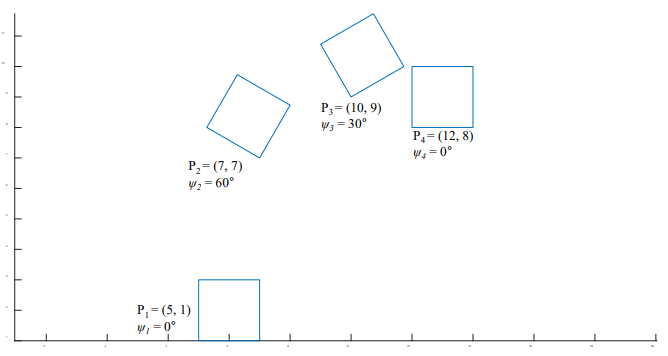
\includegraphics[width=0.7\textwidth]{MG_1.png}
    \caption{Precision Points for Motion Generation}
\end{figure}
\begin{figure}[h!]
    \centering
    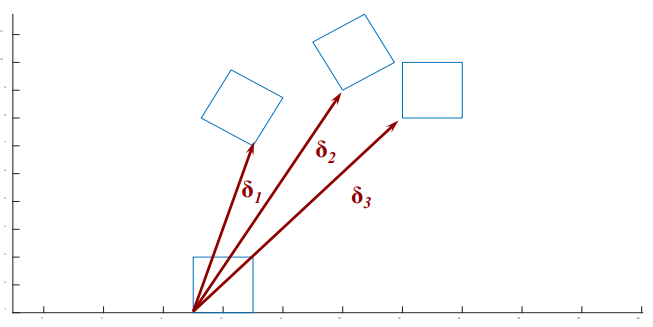
\includegraphics[width=0.7\textwidth]{MG_2.png}
    \caption{Motion Relative to First Precision Point}
\end{figure}
Now, the motion relative to the first precision point is determined such that $\delta_j$ is the position of $P_j$ relative to $P_1$, and $\alpha_j$ is the rotation of the box on $P_j$ relative to $P_1$. 

So, we have:
\begin{align}
    \delta_j&=P_j-P_1\\
    \alpha_j&=\Psi_j-\Psi_1
\end{align}

Consequently, the problem is set up and all the parameters are defined as shown in figure \ref{fig:MG_3}

\begin{figure}[h!]
    \centering
    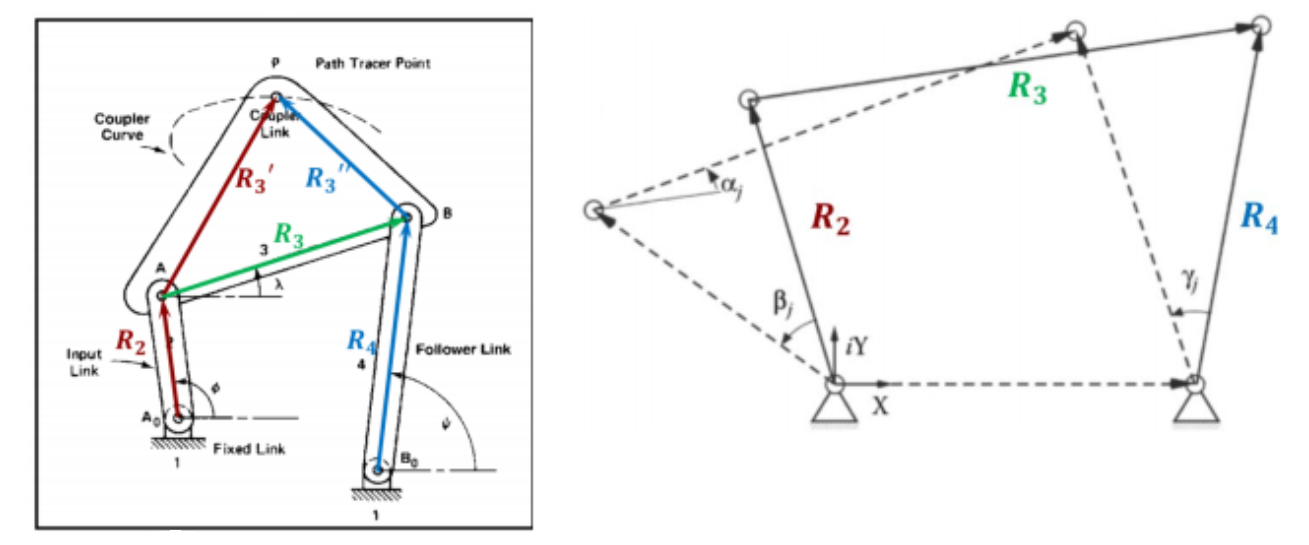
\includegraphics[width=0.7\textwidth]{MG_3.png}
    \caption{Relative and Vector Representation between Precision Points}
    \label{fig:MG_3}
\end{figure}
For motion generation, the left and right side of the system will be solved independently.

For the left side analysis,
\begin{figure}
    \centering
    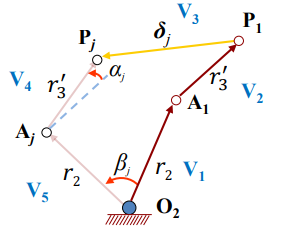
\includegraphics{MG_4.png}
    \caption{Left Side Analysis}
\end{figure}
We determine the closed-loop vector equation for the system which is as follows:
\begin{equation}
    V_1+V_2+V_3-V_4-V_5=0
\end{equation}
From this, we break down the system in terms of x and y to obtain equations \ref{eq:left_1} and \ref{eq:left_2}. Here, $\delta_j$ and $\alpha_j$ are known for $j = 1, 2, 3$ and $r_{2x}, r_{2y}, r’_{3x}, r’_{3y}$ and $\beta_j (for j = 1, 2, 3)$ are unknown. 
As we have 3 sets of equations all going to zero, the objective function can be established as seen in equation \ref{eq:left_obj}.
\begin{align}
    f_{jx}&=\color{red}r_{2x}\color{black}+\color{red}r'_{3x}\color{black}+\color{blue}\delta_{jx}\color{black}-\color{red}r'_{3x}\color{black}cos(\color{blue}\alpha_j\color{black})+\color{red}r'_{3y}\color{black}sin(\color{blue}\alpha_j\color{black})-\color{red}r_{2x}\color{black}cos(\color{red}\beta_j\color{black})+\color{red}r_{2y}\color{black}sin(\color{red}\beta_j\color{black})=0\label{eq:left_1}\\
    f_{jy}&=\color{red}r_{2y}\color{black}+\color{red}r'_{3y}\color{black}+\color{blue}\delta_{jy}\color{black}-\color{red}r'_{3y}\color{black}cos(\color{blue}\alpha_j\color{black})+\color{red}r'_{3x}\color{black}sin(\color{blue}\alpha_j\color{black})-\color{red}r_{2y}\color{black}cos(\color{red}\beta_j\color{black})+\color{red}r_{2x}\color{black}sin(\color{red}\beta_j\color{black})=0\label{eq:left_2}\\
    F&=\sqrt{(f_{1x})^2+(f_{1y})^2+(f_{2x})^2+(f_{2y})^2+(f_{3x})^2+(f_{3y})^2}\label{eq:left_obj}
\end{align}
Similarly, for right-side analysis, we arrive on the following equations:
\begin{align}
    g_{jx}&=\color{red}r_{4x}\color{black}+\color{red}r''_{3x}\color{black}+\color{blue}\delta_{jx}\color{black}-\color{red}r''_{3x}\color{black}cos(\color{blue}\alpha_j\color{black})+\color{red}r''_{3y}\color{black}sin(\color{blue}\alpha_j\color{black})-\color{red}r_{4x}\color{black}cos(\color{red}\beta_j\color{black})+\color{red}r_{4y}\color{black}sin(\color{red}\beta_j\color{black})=0\\
    g_{jy}&=\color{red}r_{4y}\color{black}+\color{red}r''_{3y}\color{black}+\color{blue}\delta_{jy}\color{black}-\color{red}r''_{3y}\color{black}cos(\color{blue}\alpha_j\color{black})+\color{red}r''_{3x}\color{black}sin(\color{blue}\alpha_j\color{black})-\color{red}r_{4y}\color{black}cos(\color{red}\beta_j\color{black})+\color{red}r_{4x}\color{black}sin(\color{red}\beta_j\color{black})=0\\
    G&=\sqrt{(g_{1x})^2+(g_{1y})^2+(g_{2x})^2+(g_{2y})^2+(g_{3x})^2+(g_{3y})^2}
\end{align}
The given ‘MSE\_211\_Lab\_2\_motion\_generation.m’ MATLAB code is used to input the different variables and equations for both left and right-side analysis, to minimize the objective functions and therefore animate the system.
\subsubsection{Path Generation}
Matlab was used to find the optimal dimensions and configuration of a 4-bar system acting as a walking spider, where the tip of the leg must pass through four precision points as a function of the input angle, a diagram of these points can be seen in figure \ref{fig:precionpoints_PG}.

\begin{figure}[H]
    \centering
    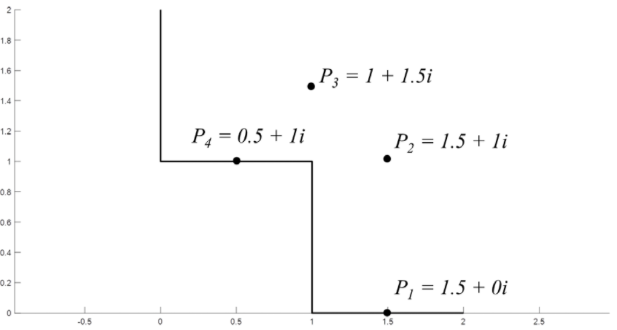
\includegraphics[width=0.7\textwidth]{path_generation.png}
    \caption{Precision Point for Path Generation}
    \label{fig:precionpoints_PG}
\end{figure}
To find the optimal dimensions, a system of loop equations of the vector representations of the bars and relative angles between them were assembled and placed into a objective function to be minimized by a minimizing function in Matlab. This method was performed from the left and right side, shown in the figures below are the general structure of the left side analysis loop equations and the objective function, the red text are the unknown variables.
\begin{align}
    f_{jx}&=\color{red}r_{2x}\color{black}+\color{red}r'_{3x}\color{black}+\color{blue}\delta_{jx}\color{black}-\color{red}r'_{3x}\color{black}cos(\color{red}\alpha_j\color{black})+\color{red}r'_{3y}\color{black}sin(\color{red}\alpha_j\color{black})-\color{red}r_{2x}\color{black}cos(\color{blue}\beta_j\color{black})+\color{red}r_{2y}\color{black}sin(\color{blue}\beta_j\color{black})=0\\
    f_{jy}&=\color{red}r_{2y}\color{black}+\color{red}r'_{3y}\color{black}+\color{blue}\delta_{jy}\color{black}-\color{red}r'_{3y}\color{black}cos(\color{red}\alpha_j\color{black})+\color{red}r'_{3x}\color{black}sin(\color{red}\alpha_j\color{black})-\color{red}r_{2y}\color{black}cos(\color{blue}\beta_j\color{black})+\color{red}r_{2x}\color{black}sin(\color{blue}\beta_j\color{black})=0\\
    F&=\sqrt{(f_{1x})^2+(f_{1y})^2+(f_{2x})^2+(f_{2y})^2+(f_{3x})^2+(f_{3y})^2}
\end{align}

\subsubsection{Function Generation}
The function generation method allows a continuous output based on input, primarily the input and output angles are known, and the required movement of the mechanism are to be calculated. For the purpose of this lab the movement of joint are specified, the input must travel 60 degrees and the output travels at 90 degrees.

\begin{figure}[h!]
    \centering
    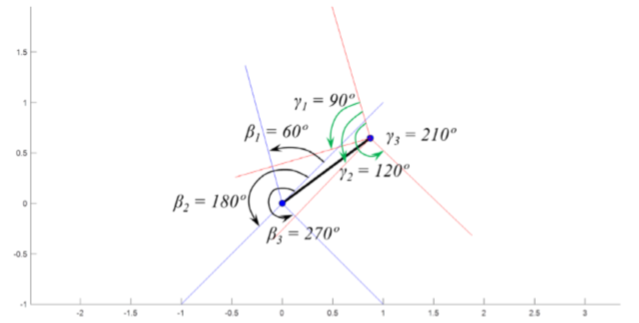
\includegraphics[width=0.7\textwidth]{func_gen.png}
    \caption{Precision Point for Function Generation}
    \label{fig:precisionpoint_FG}
\end{figure}
The equation associated with each of the linkage movements are defined but the j is varied in the code.
\begin{multline}
    f_{jx}=-\color{blue}r_{2x}\color{black}cos(\color{blue}\beta_j\color{black})+\color{blue}r_{2y}\color{black}sin(\color{blue}\beta_j\color{black})-\color{red}r_{3x}\color{black}cos(\color{red}\phi_{j}\color{black})+\color{red}r_{3y}\color{black}sin(\color{red}\phi_j\color{black})+\\\color{red}r_{4x}\color{black}cos(\color{blue}\gamma_{j}\color{black})-\color{red}r_{4y}\color{black}sin(\color{blue}\gamma_{j}\color{black})+\color{blue}r_{2x}\color{black}+\color{red}r_{3x}\color{black}-\color{red}r_{4x}\color{black}=0
\end{multline}
\begin{multline}
    f_{jy}=-\color{blue}r_{2x}\color{black}sin(\color{blue}\beta_j\color{black})+\color{blue}r_{2y}\color{black}cos(\color{blue}\beta_j\color{black})-\color{red}r_{3x}\color{black}sin(\color{red}\phi_{j}\color{black})+\color{red}r_{3y}\color{black}cos(\color{red}\phi_j\color{black})+\\\color{red}r_{4x}\color{black}sin(\color{blue}\gamma_{j}\color{black})-\color{red}r_{4y}\color{black}cos(\color{blue}\gamma_{j}\color{black})+\color{blue}r_{2x}\color{black}+\color{red}r_{3x}\color{black}-\color{red}r_{4x}\color{black}=0
\end{multline}
\begin{equation}
        F=\sqrt{(f_{1x})^2+(f_{1y})^2+(f_{2x})^2+(f_{2y})^2+(f_{3x})^2+(f_{3y})^2}
\end{equation}

\pagebreak
\section{Results}
\subsection{Part 1}
\subsubsection{Steepest Decent Method}
Show in table \ref{tab:SDM_guess1} to \ref{tab:SDM_guess4} are several iterations of the steepest decent method with different starting guesses. We found the steepest decent method to be very reliable and to always converge on a minima. We also saw the importance of the starting guess. In this case where we had a graphical representation of the function, it was relatively easy to choose a good starting guess. However if we did not have a contour graph we would have to randomly choose starting points and hope that the algorithm would converge to all the points we are interested in. The code for this method can be found in appendix \ref{list:part1}.
% Table generated by Excel2LaTeX from sheet 'Guess1_SDM'
\begin{table}[h!]
  \centering
  \caption{Steepest Decent with $(x_i,y_i) = (0,0)$}
    \begin{tabular}{rrrrr}
    \multicolumn{1}{l}{\textbf{Iteration}} & \multicolumn{1}{l}{\textbf{Estimated Point X}} & \multicolumn{1}{l}{\textbf{Estimated Point Y}} & \multicolumn{1}{l}{\textbf{F(x,y)}} & \multicolumn{1}{l}{\textbf{Error}} \\
    1     & 0.013 & 0.020 & 170.000 & \multicolumn{1}{l}{NaN} \\
    11    & 0.178 & 0.259 & 161.528 & 0.033 \\
    21    & 0.468 & 0.619 & 143.939 & 0.057 \\
    31    & 2.545 & 2.230 & 5.863 & 0.767 \\
    41    & 2.659 & 2.224 & 3.439 & 0.010 \\
    51    & 2.735 & 2.212 & 2.193 & 0.007 \\
    61    & 2.790 & 2.197 & 1.475 & 0.005 \\
    71    & 2.831 & 2.182 & 1.032 & 0.004 \\
    81    & 2.862 & 2.166 & 0.744 & 0.003 \\
    91    & 2.886 & 2.151 & 0.548 & 0.003 \\
    101   & 2.905 & 2.137 & 0.412 & 0.002 \\
    111   & 2.921 & 2.124 & 0.313 & 0.002 \\
    121   & 2.933 & 2.111 & 0.241 & 0.002 \\
    131   & 2.943 & 2.100 & 0.186 & 0.001 \\
    141   & 2.952 & 2.090 & 0.145 & 0.001 \\
    151   & 2.958 & 2.080 & 0.113 & 0.001 \\
    \textbf{159} & \textbf{2.963} & \textbf{2.073} & \textbf{0.090} & \textbf{0.001} \\
    \end{tabular}%
  \label{tab:SDM_guess1}%
\end{table}%

% Table generated by Excel2LaTeX from sheet 'Guess2_SDM'
\begin{table}[h!]
  \centering
  \caption{Steepest Decent with $(x_i,y_i) = (-1,0)$}
    \begin{tabular}{rrrrr}
    \multicolumn{1}{l}{\textbf{Iteration}} & \multicolumn{1}{l}{\textbf{Estimated Point X}} & \multicolumn{1}{l}{\textbf{Estimated Point Y}} & \multicolumn{1}{l}{\textbf{F(x,y)}} & \multicolumn{1}{l}{\textbf{Error}} \\
    1     & -1.027 & 0.023 & 164.000 & \multicolumn{1}{l}{NaN} \\
    11    & -1.428 & 0.363 & 146.128 & 0.069 \\
    21    & -2.898 & 2.899 & 53.421 & 0.209 \\
    31    & -2.885 & 2.933 & 1.756 & 0.004 \\
    41    & -2.874 & 2.963 & 1.286 & 0.003 \\
    51    & -2.864 & 2.988 & 0.944 & 0.003 \\
    61    & -2.856 & 3.009 & 0.693 & 0.002 \\
    71    & -2.849 & 3.027 & 0.510 & 0.002 \\
    81    & -2.844 & 3.042 & 0.375 & 0.002 \\
    91    & -2.839 & 3.055 & 0.276 & 0.001 \\
    101   & -2.834 & 3.066 & 0.203 & 0.001 \\
    \textbf{108} & \textbf{-2.832} & \textbf{3.073} & \textbf{0.159} & \textbf{0.001} \\
    \end{tabular}%
  \label{tab:SDM_gess2}%
\end{table}%

% Table generated by Excel2LaTeX from sheet 'Guess3_SDM'
\begin{table}[h!]
  \centering
  \caption{Steepest Decent with $(x_i,y_i) = (0,-1)$}
    \begin{tabular}{rrrrr}
    \multicolumn{1}{l}{\textbf{Iteration}} & \multicolumn{1}{l}{\textbf{Estimated Point X}} & \multicolumn{1}{l}{\textbf{Estimated Point Y}} & \multicolumn{1}{l}{\textbf{F(x,y)}} & \multicolumn{1}{l}{\textbf{Error}} \\
    1     & 0.019 & -1.000 & 180.000 & \multicolumn{1}{l}{NaN} \\
    11    & 0.321 & -0.991 & 174.871 & 0.039 \\
    21    & 1.141 & -0.952 & 146.080 & 0.120 \\
    31    & 3.527 & -1.212 & 4.315 & 0.118 \\
    41    & 3.539 & -1.351 & 2.804 & 0.011 \\
    51    & 3.546 & -1.432 & 2.051 & 0.007 \\
    61    & 3.552 & -1.491 & 1.558 & 0.005 \\
    71    & 3.556 & -1.537 & 1.208 & 0.004 \\
    81    & 3.559 & -1.576 & 0.949 & 0.004 \\
    91    & 3.562 & -1.608 & 0.752 & 0.003 \\
    101   & 3.565 & -1.635 & 0.600 & 0.003 \\
    111   & 3.567 & -1.658 & 0.482 & 0.002 \\
    121   & 3.569 & -1.679 & 0.388 & 0.002 \\
    131   & 3.571 & -1.696 & 0.314 & 0.002 \\
    141   & 3.572 & -1.712 & 0.254 & 0.002 \\
    151   & 3.573 & -1.726 & 0.207 & 0.001 \\
    161   & 3.574 & -1.738 & 0.168 & 0.001 \\
    171   & 3.575 & -1.749 & 0.137 & 0.001 \\
    \textbf{175} & \textbf{3.576} & \textbf{-1.753} & \textbf{0.124} & \textbf{0.001} \\
    \end{tabular}%
  \label{tab:SDM_guess3}%
\end{table}%

% Table generated by Excel2LaTeX from sheet 'Guess4_SDM'
\begin{table}[h!]
  \centering
  \caption{Steepest Decent with $(x_i,y_i) = (-1,-1)$}
    \begin{tabular}{rrrrr}
    \multicolumn{1}{l}{\textbf{Iteration}} & \multicolumn{1}{l}{\textbf{Estimated Point X}} & \multicolumn{1}{l}{\textbf{Estimated Point Y}} & \multicolumn{1}{l}{\textbf{F(x,y)}} & \multicolumn{1}{l}{\textbf{Error}} \\
    1     & -1.055 & -1.011 & 170.000 & \multicolumn{1}{l}{NaN} \\
    11    & -2.691 & -1.582 & 85.692 & 0.102 \\
    21    & -3.719 & -2.859 & 6.643 & 0.005 \\
    31    & -3.712 & -2.906 & 5.281 & 0.004 \\
    41    & -3.709 & -2.946 & 4.245 & 0.004 \\
    51    & -3.708 & -2.981 & 3.443 & 0.003 \\
    61    & -3.708 & -3.011 & 2.814 & 0.003 \\
    71    & -3.709 & -3.038 & 2.313 & 0.003 \\
    81    & -3.711 & -3.061 & 1.912 & 0.002 \\
    91    & -3.714 & -3.082 & 1.587 & 0.002 \\
    101   & -3.716 & -3.101 & 1.322 & 0.002 \\
    111   & -3.719 & -3.117 & 1.106 & 0.002 \\
    121   & -3.722 & -3.132 & 0.927 & 0.001 \\
    131   & -3.725 & -3.145 & 0.779 & 0.001 \\
    141   & -3.728 & -3.157 & 0.657 & 0.001 \\
    151   & -3.731 & -3.168 & 0.555 & 0.001 \\
    \textbf{158} & \textbf{-3.733} & \textbf{-3.175} & \textbf{0.485} & \textbf{0.001} \\
    \end{tabular}%
  \label{tab:SDM_guess4}%
\end{table}%

\begin{landscape}
\begin{figure}[h!]
    \centering
    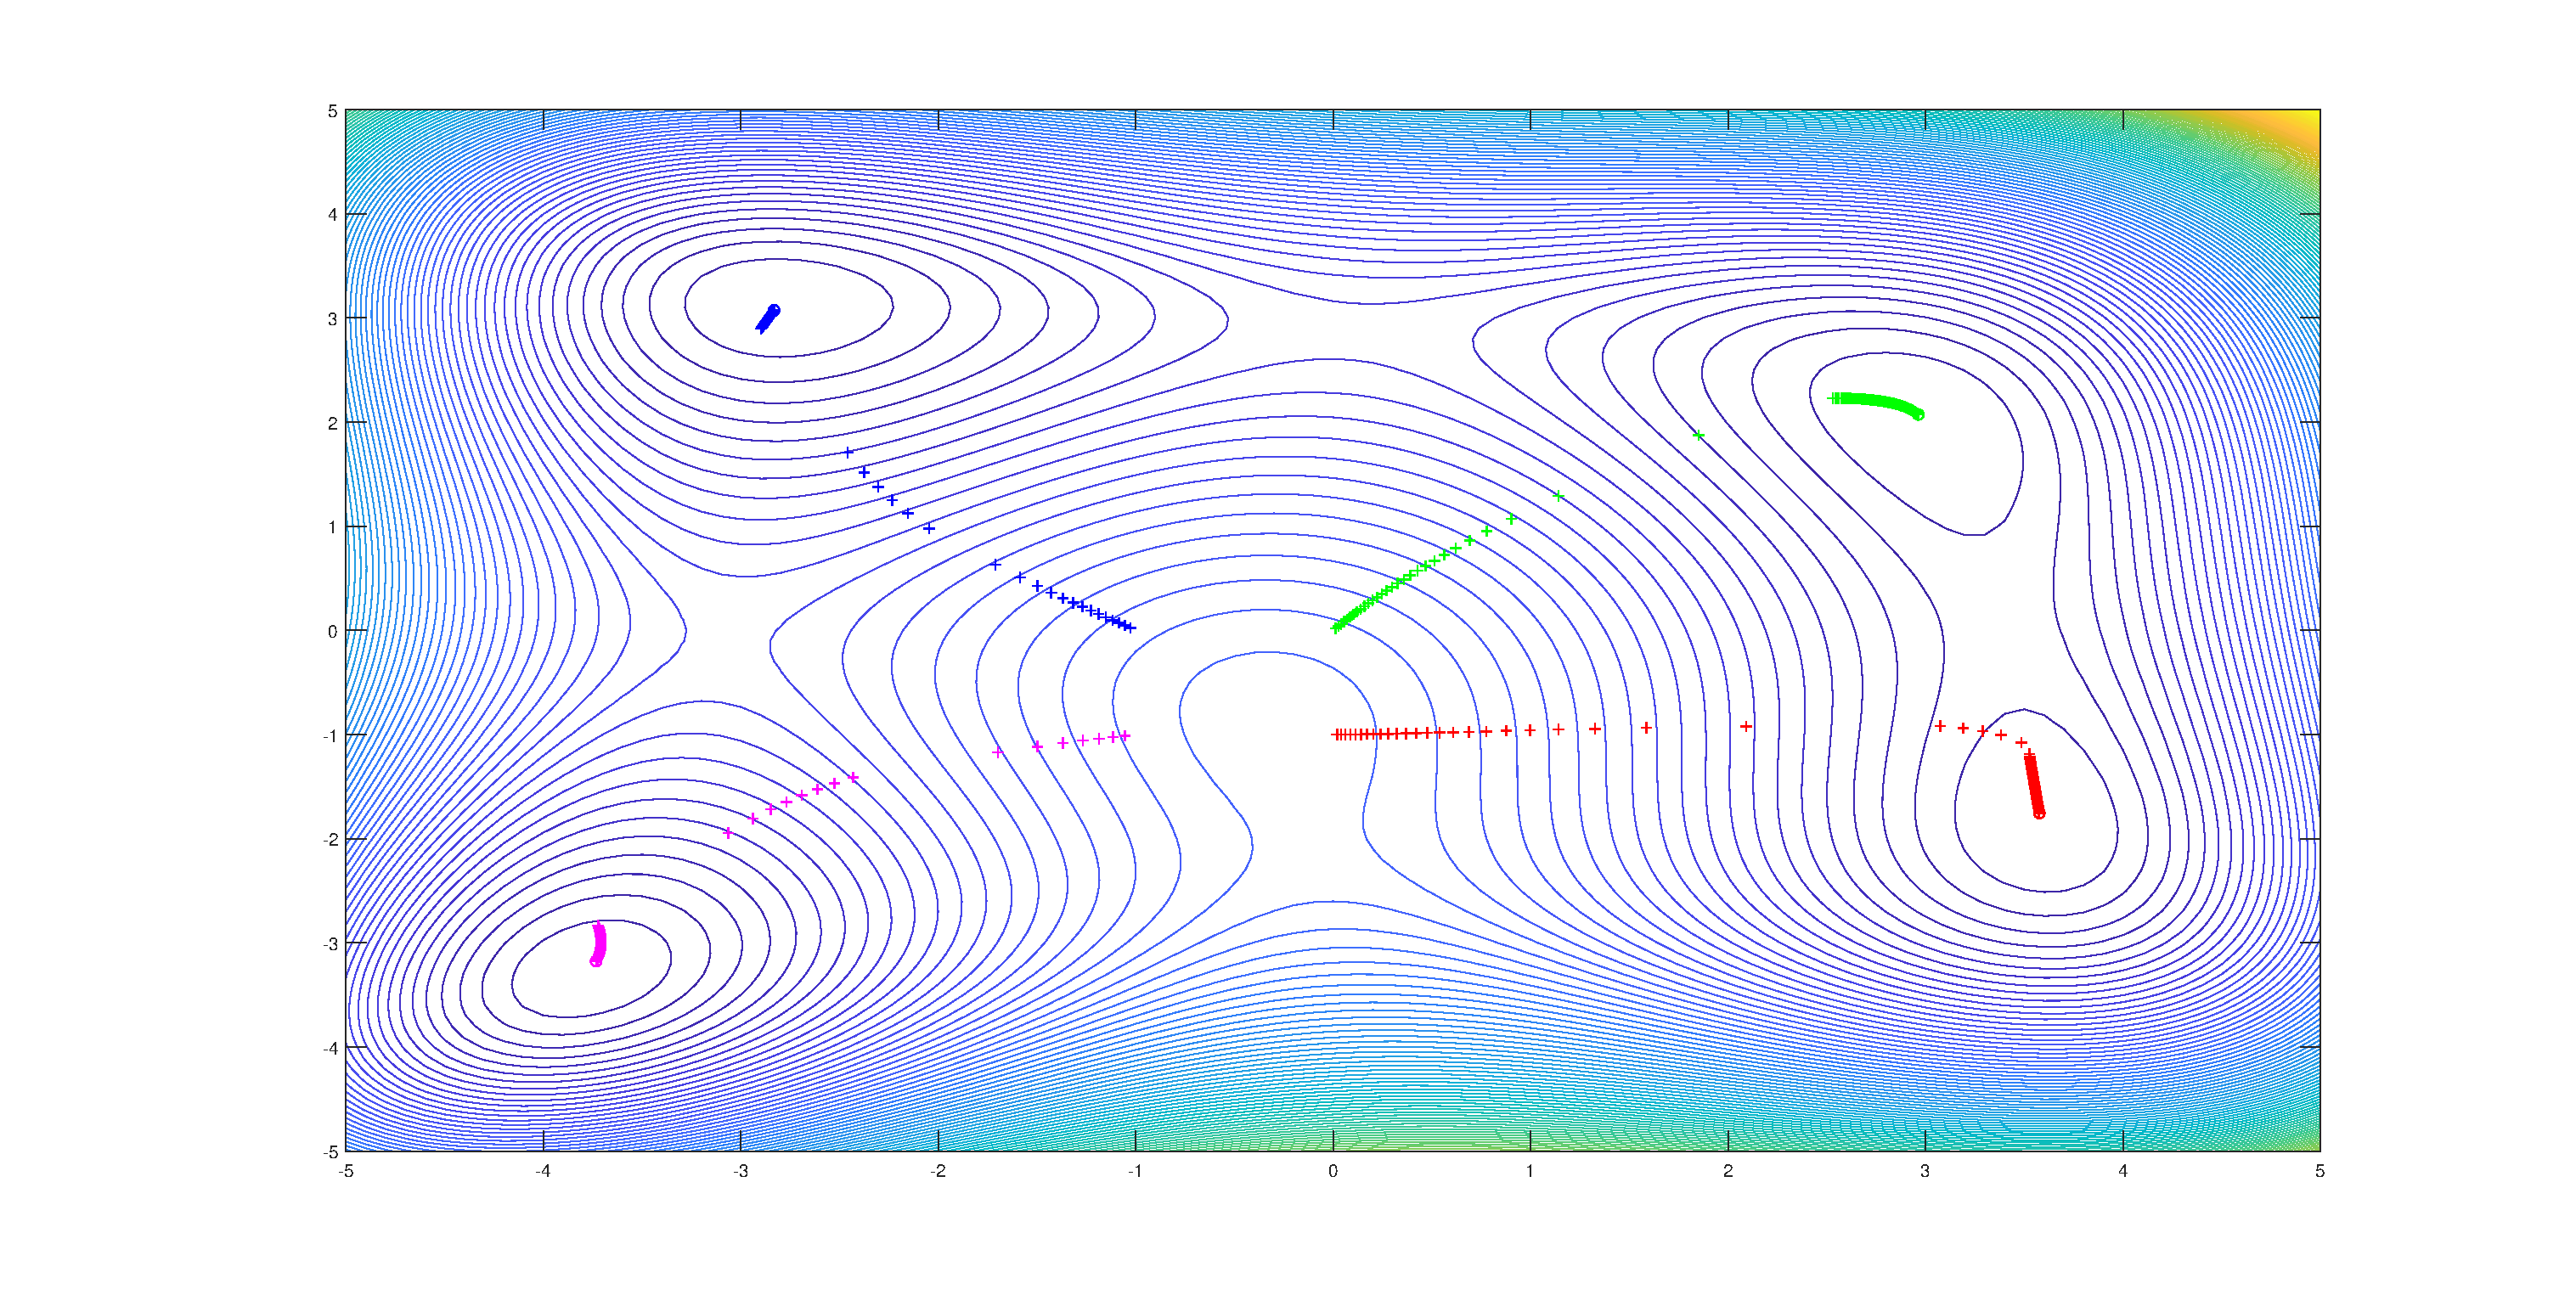
\includegraphics[width=9in,height=6.5in]{SDM_Contour.eps}
    \caption{Contour Plot with Steepest Decent}
    \label{fig:SDM_Contour}
\end{figure}
\end{landscape}
\pagebreak
\subsubsection{Newton's Method}
When implementing Newton's method we encountered problems with using the same guesses as the steepest decent method. When we use the initial points from SDM the algorithm does not converge to a minima, however if we choose initial points closer to the minima, the algorithm quickly converges to the correct point.
% Table generated by Excel2LaTeX from sheet 'Sheet1'
\begin{table}[h!]
  \centering
  \caption{Newton's Method with $(x_i,y_i) = (0,0)$}
    \begin{tabular}{rrrrr}
    \multicolumn{1}{l}{\textbf{Iteration }} & \multicolumn{1}{l}{\textbf{Estimated Point X}} & \multicolumn{1}{l}{\textbf{Estimated Point Y}} & \multicolumn{1}{l}{\textbf{F(x,y)}} & \multicolumn{1}{l}{\textbf{Error}} \\
    1     & 0.000 & 0.000 & 170.000 & \multicolumn{1}{l}{NaN} \\
    2     & -0.333 & -0.846 & 181.501 & 0.909 \\
    3     & -0.271 & -0.919 & 181.616 & 0.096 \\
    4     & -0.271 & -0.923 & 181.617 & 0.004 \\
    5     & -0.271 & -0.923 & 181.617 & 0.000 \\
    \end{tabular}%
\end{table}%
% Table generated by Excel2LaTeX from sheet 'Sheet1'
\begin{table}[h!]
  \centering
  \caption{Newton's Method with $(x_i,y_i) = (-1,0)$}
    \begin{tabular}{rrrrr}
    \multicolumn{1}{l}{\textbf{Iteration }} & \multicolumn{1}{l}{\textbf{Estimated Point X}} & \multicolumn{1}{l}{\textbf{Estimated Point Y}} & \multicolumn{1}{l}{\textbf{F(x,y)}} & \multicolumn{1}{l}{\textbf{Error}} \\
    1     & -1.000 & 0.000 & 164.000 & \multicolumn{1}{l}{NaN} \\
    2     & -0.095 & -0.787 & 180.656 & 1.200 \\
    3     & -0.273 & -0.921 & 181.616 & 0.222 \\
    4     & -0.271 & -0.923 & 181.617 & 0.003 \\
    5     & -0.271 & -0.923 & 181.617 & 0.000 \\
    \end{tabular}%
\end{table}%
% Table generated by Excel2LaTeX from sheet 'Sheet1'
\begin{table}[h!]
  \centering
  \caption{Newton's Method with $(x_i,y_i) = (-3,-3)$}
    \begin{tabular}{rrrrr}
    \multicolumn{1}{l}{\textbf{Iteration }} & \multicolumn{1}{l}{\textbf{Estimated Point X}} & \multicolumn{1}{l}{\textbf{Estimated Point Y}} & \multicolumn{1}{l}{\textbf{F(x,y)}} & \multicolumn{1}{l}{\textbf{Error}} \\
    1     & -3.000 & -3.000 & 26.000 & \multicolumn{1}{l}{NaN} \\
    2     & -4.282 & -3.468 & 15.523 & 1.365 \\
    3     & -3.858 & -3.313 & 0.342 & 0.452 \\
    4     & -3.782 & -3.284 & 0.000 & 0.082 \\
    5     & -3.779 & -3.283 & 0.000 & 0.003 \\
    6     & -3.779 & -3.283 & 0.000 & 0.000 \\
    \end{tabular}%
\end{table}%
% Table generated by Excel2LaTeX from sheet 'Sheet1'
\begin{table}[H]
  \centering
  \caption{Newton's Method with $(x_i,y_i) = (3,-3)$}
    \begin{tabular}{rrrrr}
    \multicolumn{1}{l}{\textbf{Iteration }} & \multicolumn{1}{l}{\textbf{Estimated Point X}} & \multicolumn{1}{l}{\textbf{Estimated Point Y}} & \multicolumn{1}{l}{\textbf{F(x,y)}} & \multicolumn{1}{l}{\textbf{Error}} \\
    1     & 3.000 & -3.000 & 50.000 & \multicolumn{1}{l}{NaN} \\
    2     & 3.926 & -2.255 & 8.705 & 1.188 \\
    3     & 3.627 & -1.943 & 0.209 & 0.432 \\
    4     & 3.586 & -1.855 & 0.001 & 0.098 \\
    5     & 3.584 & -1.848 & 0.000 & 0.007 \\
    6     & 3.584 & -1.848 & 0.000 & 0.000 \\
    \end{tabular}%
\end{table}%
\begin{landscape}
\begin{figure}[h!]
    \centering
    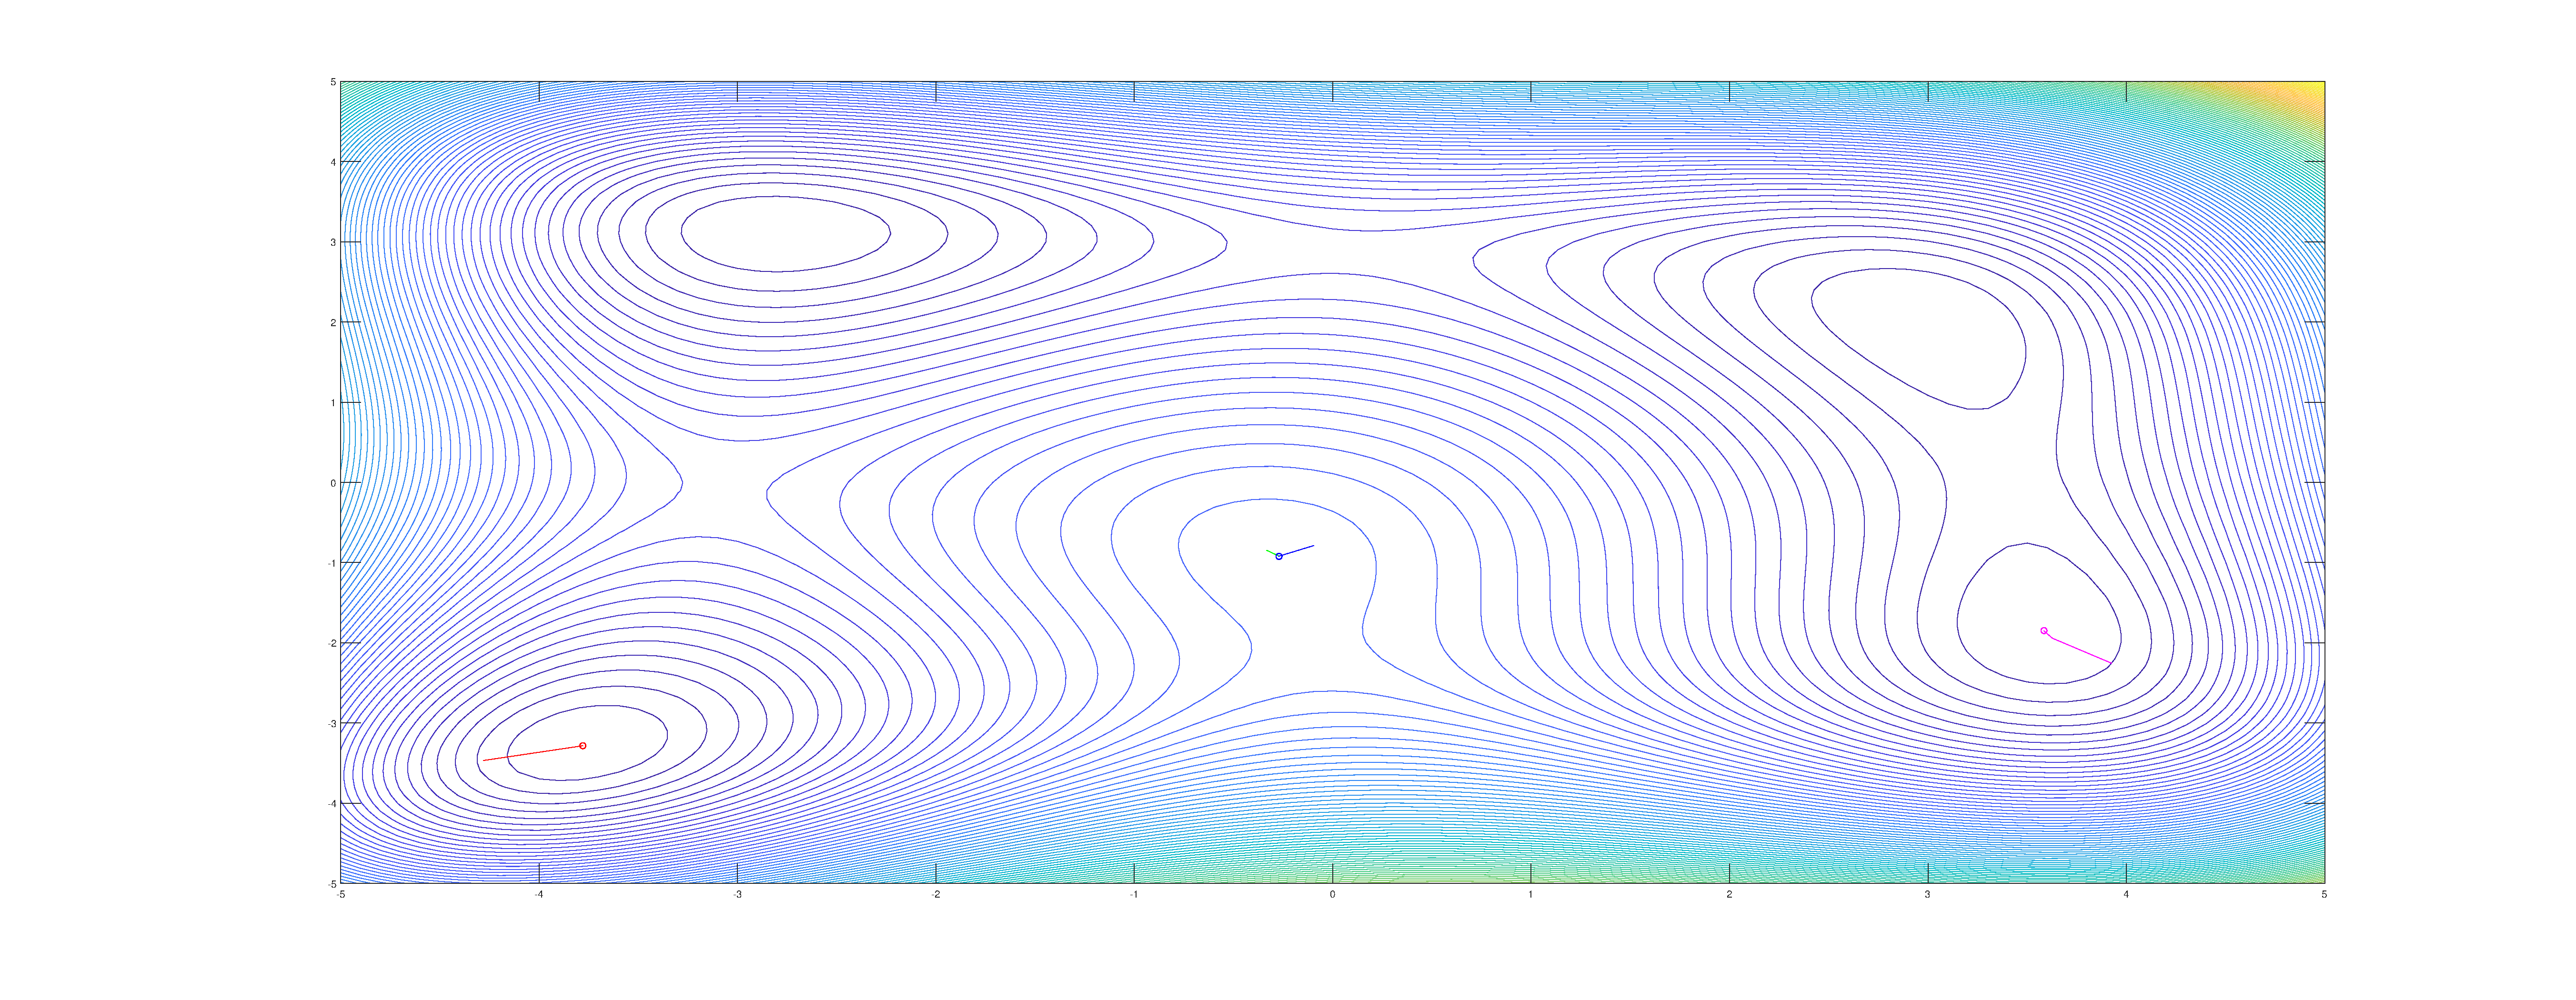
\includegraphics[width=9in,height=6.5in]{NM_Contour.eps}
    \caption{Contour Plot with Newton's Method}
    \label{fig:SDM_Contour}
\end{figure}
\end{landscape}

\subsubsection{Matlab's Function}
From table \ref{tab:fminunc} we can see that MATLAB's function find the minima much quicker than the steepest decent method and reliably converges.
% Table generated by Excel2LaTeX from sheet 'Sheet1'
\begin{table}[htbp]
  \centering
  \caption{\textit{fminunc} With Different Initial Guess}
    \begin{tabular}{lrrrr}
    \textbf{Initial Guess} & \multicolumn{1}{l}{\textbf{\# Iterations}} & \multicolumn{1}{l}{\textbf{Estimated X Point}} & \multicolumn{1}{l}{\textbf{Estimated Y Point}} & \multicolumn{1}{l}{\textbf{F(x,y)}} \\
    (0,0) & 9     & 3.000 & 2.000 & 1.67E-13 \\
    (-1,0) & 8     & -2.805 & 3.131 & 1.00E-13 \\
    (0,-1) & 8     & 3.584 & -1.848 & 7.05E-13 \\
    (-1,-1) & 9     & -3.779 & -3.283 & 5.21E-13 \\
    \end{tabular}%
  \label{tab:fminunc}%
\end{table}%

\subsection{Part 2}
\subsubsection{Motion Generation}
The position and rotation of the precision points are put in as follows:
\begin{figure}[h!]
    \centering
    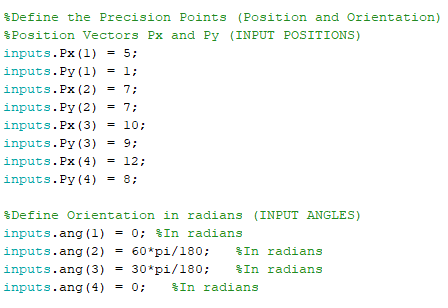
\includegraphics[width=0.7\textwidth]{MG_5.png}
\end{figure}

Consequently, the respective known parameters, i.e $\delta_i$ and $\alpha_i$ are determined.The initial values are then determined through trial and error, by first analyzing the respective quadrant of the element, and the position and orientation of the precision points.
\begin{figure}[h!]
    \centering
    \begin{minipage}{.5\textwidth}
        \centering
        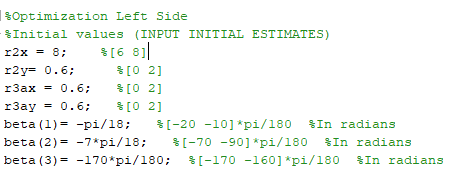
\includegraphics[width=1\textwidth]{MG_6.png}
    \end{minipage}%
    \begin{minipage}{0.5\textwidth}
        \centering
        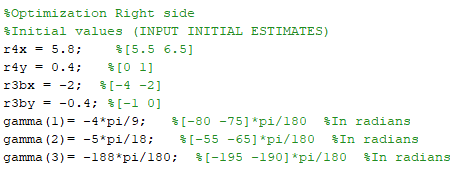
\includegraphics[width=1\textwidth]{MG_7.png}
    \end{minipage}
\end{figure}

The relative equations for each precision point are set up for left and right-side analysis, using the equations mentioned above and the objective functions for both cases are determined. Consequently, the optimization algorithm is called via the ‘left side’ and ‘right side’ functions and the initial estimates.The function evaluation limit of 700 was reached and the values were determined to a reasonable accuracy.
% Table generated by Excel2LaTeX from sheet 'Sheet1'
\begin{table}[H]
  \centering
  \caption{Lengths of Links Motion Generation}
    \begin{tabular}{cccc}
    \textbf{r1}    & \textbf{r2}    & \textbf{r3}    & \textbf{r4} \\
    8.226 & 5.672 & 7.610 & 4.984 \\
    \end{tabular}%
\end{table}%
\begin{figure}[H]
    \centering
    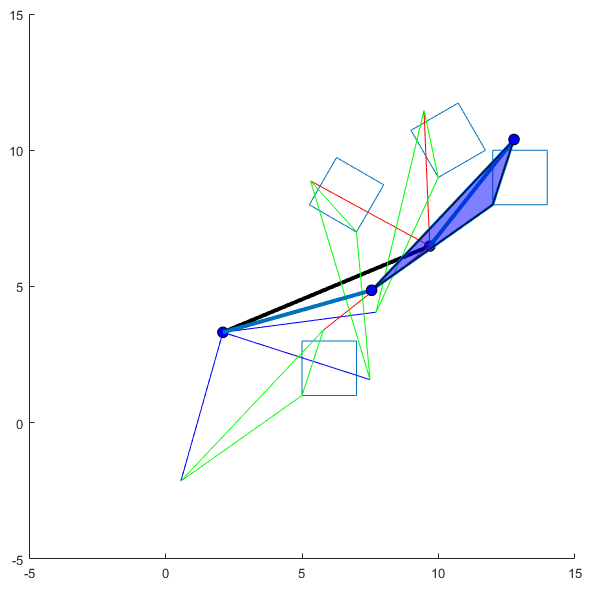
\includegraphics[width=0.7\textwidth,height=3in]{MG_8.png}
    \caption{Motion Generation Animation}
\end{figure}

\subsubsection{Path Generation}
The initial values were again found by a brute-force trial and error method, the signs of the variables were honed in on by observing which quadrant the resultant simulation was in, the decided first estimates for the left and right sides can be seen respectively in the figure below.
\begin{figure}[H]
    \centering
    \begin{minipage}{.5\textwidth}
        \centering
        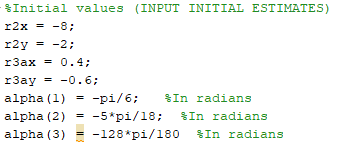
\includegraphics[width=1\textwidth]{PG_1.png}
    \end{minipage}%
    \begin{minipage}{0.5\textwidth}
        \centering
        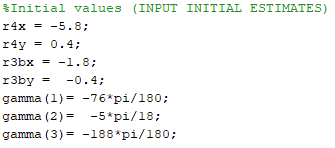
\includegraphics[width=1\textwidth]{PG_2.png}
    \end{minipage}
\end{figure}

Inputting these variables into a minimizing function, values were found and then placed in objective functions to confirm their efficacy, the function iterated to its max amount of function evaluations of 700.The Matlab code then outputted a animation and the values of the dimensions of the mechanism. Which can be seen in figure \ref{fig:PG_animation}.The accuracy of this method was relatively accurate, as objective functions were 0 to 5 decimal places, and gave a solution relatively fast.

% Table generated by Excel2LaTeX from sheet 'Sheet1'
\begin{table}[H]
  \centering
  \caption{Lengths of Links Path Generation}
    \begin{tabular}{cccc}
    \textbf{r1}    & \textbf{r2}    & \textbf{r3}    & \textbf{r4} \\
    0.497 & 0.707 & 0.472 & 0.773 \\
    \end{tabular}%
\end{table}%
\begin{figure}[H]
    \centering
    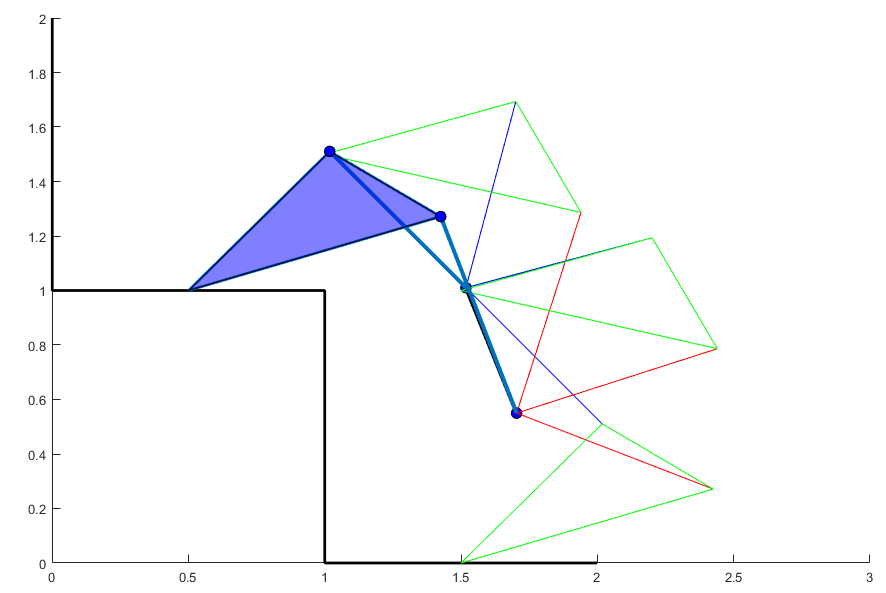
\includegraphics[width=0.7\textwidth]{PG_3.png}
    \caption{Path Generation Animation}
    \label{fig:PG_animation}
\end{figure}

\subsubsection{Function Generation}
The function generation successfully follows the mechanisms described in the manual. However to achieve the motion several iterations of initial guesses were needed. Primarily, a technique was tried in which the output phi reported by Matlab was input as the initial guess. However, this method was semi-success.The initial guess which successfully complete the function are shown below:
\begin{align}
    \phi_1&=-0.178\nonumber\\
    \phi_1&=-1.223\nonumber\\
    \phi_1&=-2.92\nonumber
\end{align}
% Table generated by Excel2LaTeX from sheet 'Sheet1'
\begin{table}[H]
  \centering
  \caption{Lengths of Links Function Generation}
    \begin{tabular}{cccc}
    r1    & r2    & r3    & r4 \\
    1.048 & 1.414 & 1.132 & 1.344 \\
    \end{tabular}%
\end{table}%
\begin{figure}[H]
    \centering
    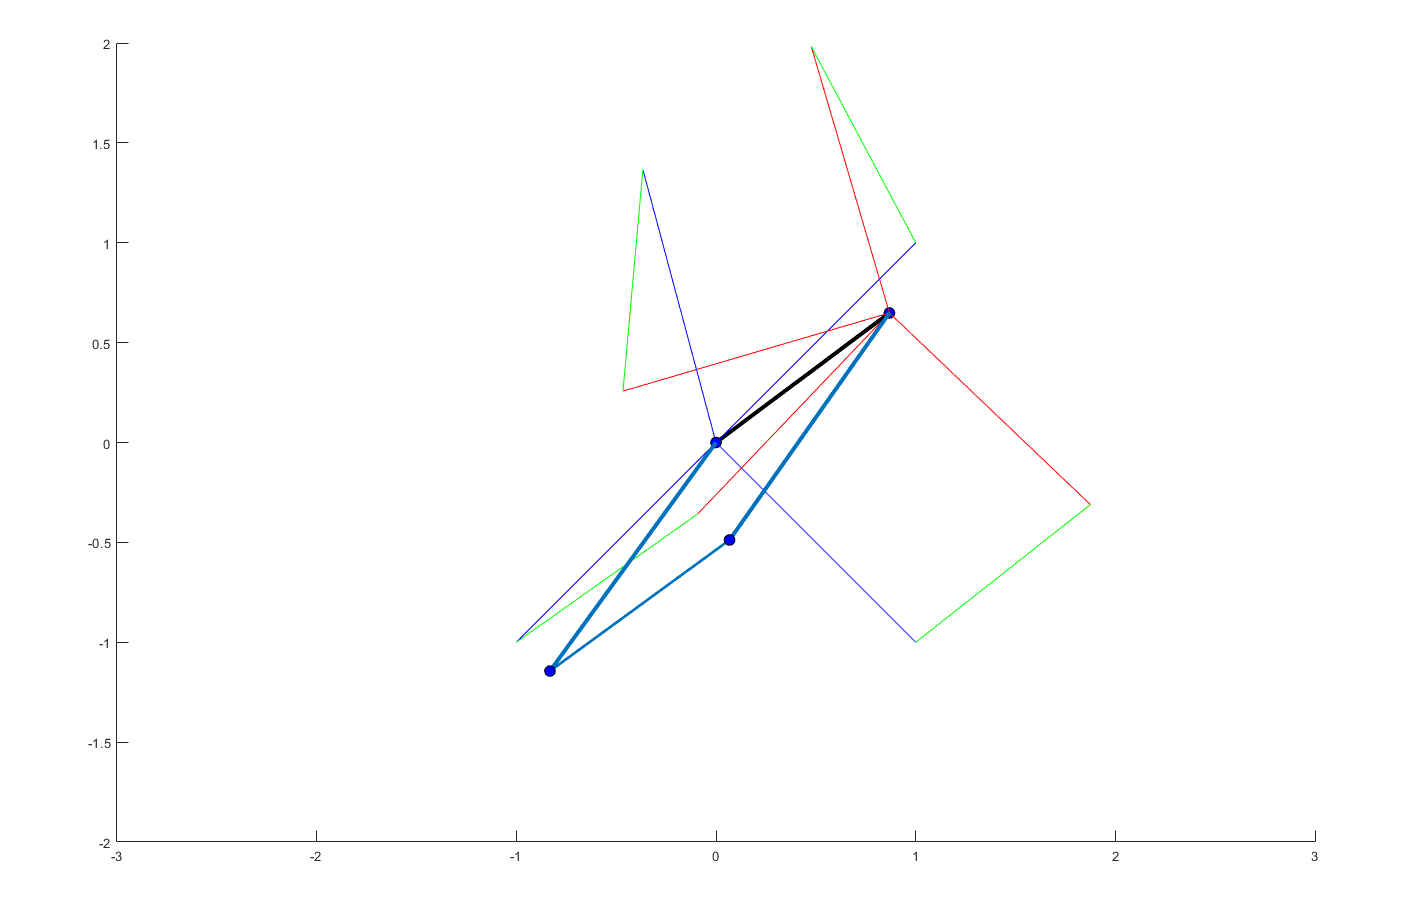
\includegraphics[width=0.7\textwidth]{FG_1.png}
    \caption{Function Generation Animation}
    \label{fig:FG_animation}
\end{figure}
As it can be seen, the four-bar links follows the angles outlined in the lab manual. 
\pagebreak
\section{Conclusion}
Overall, all of the procedure of the lab manual was followed and showed successful results. Part 1 in the Lab showed that choosing the right algorithm can save time and power to conclude the same results. Furthermore Part 2 provided the necessary equation and the methodology to execute the upcoming project. In the end, the lab provided useful skills and algorithms needed to complete future problems.
\pagebreak

\appendix
\section{Matlab Code}
\subsection{Part 1}\label{list:part1}
\lstinputlisting[style=Matlab-editor, basicstyle=\mlttfamily\scriptsize, caption={Lab\_2\_main.m}]{Part1_MatlabCode/Lab_2_main.m}
\lstinputlisting[style=Matlab-editor, basicstyle=\mlttfamily\scriptsize, caption={Lab\_2\_Fun.m}]{Part1_MatlabCode/Lab_2_Fun.m}
\lstinputlisting[style=Matlab-editor, basicstyle=\mlttfamily\scriptsize, caption={Lab\_2\_Grad.m}]{Part1_MatlabCode/Lab_2_Grad.m}
\lstinputlisting[style=Matlab-editor, basicstyle=\mlttfamily\scriptsize, caption={Lab\_2\_Hess.m}]{Part1_MatlabCode/Lab_2_Hess.m}
\lstinputlisting[style=Matlab-editor, basicstyle=\mlttfamily\scriptsize, caption={Lab\_2\_sdm.m}]{Part1_MatlabCode/Lab_2_sdm.m}
\lstinputlisting[style=Matlab-editor, basicstyle=\mlttfamily\scriptsize, caption={Lab\_2\_Newton.m}]{Part1_MatlabCode/Lab_2_Newton.m}
\pagebreak
\subsection{Part 2}
\lstinputlisting[style=Matlab-editor, basicstyle=\mlttfamily\scriptsize, caption={MSE\_211\_Lab\_2\_motion\_generation.m}]{Part2_MatlabCode/MSE_211_Lab_2_motion_generation.m}
\lstinputlisting[style=Matlab-editor, basicstyle=\mlttfamily\scriptsize, caption={MSE\_211\_Lab\_2\_path\_generation.m}]{Part2_MatlabCode/MSE_211_Lab_2_path_generation.m}
\lstinputlisting[style=Matlab-editor, basicstyle=\mlttfamily\scriptsize, caption={MSE\_211\_Lab\_2\_function\_generation.m}]{Part2_MatlabCode/MSE_211_Lab_2_function_generation.m}

\end{document}
              
            